\section{PERCEPTION}

Environment perception is a fundamental function to enable autonomous vehicles,
which provides the vehicle with crucial information on the driving environment,
including the free drivable areas and surrounding obstacles’ locations,
velocities, and even predictions of their future states. Based on the sensors
implemented, the environment perception task can be tackled by using LIDARs,
cameras, or a fusion between these two kinds of devices. Some other traditional
approaches also involve the use of short/long-range radars and ultrasonic
sensors. Regardless of the sensors being implemented, two critical elements of
the perception task are (i) road surface extraction and (ii) on-road object
detection.

\subsection{LIDAR}

LIDAR refers to a light detection and ranging device, which sends millions of
light pulses per second in a well-designed pattern. With its rotating axis, it
is able to create a dynamic, three-dimensional map of the environment. LIDAR is
the heart for object detection for most of the existing autonomous vehicles.
Figure \ref{fig:lidar} shows the ideal detection results from a 3D LIDAR, with
all the moving objects being identified.

\begin{figure}[h]
    \centering
    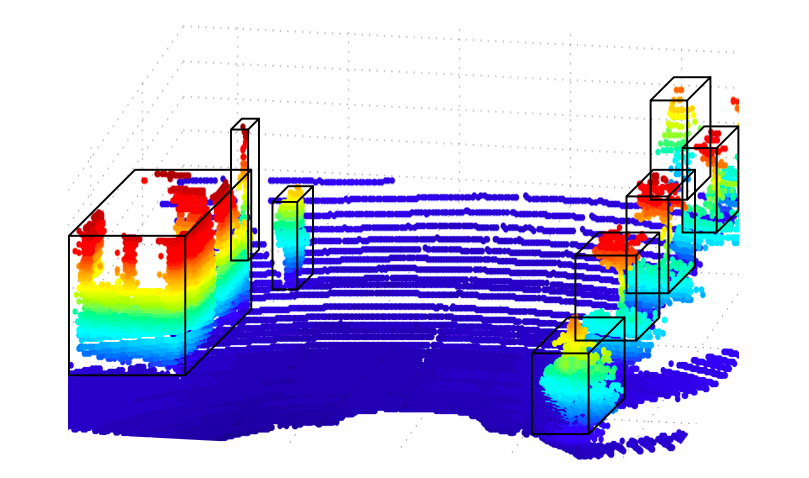
\includegraphics[width=0.5\textwidth]{lidar.png}
    \caption{The ideal detection result from a 3D LIDAR with all moving objects detected.}
    \label{fig:lidar}
\end{figure}

In a real scene, the points returned by the LIDAR are never perfect. The
difficulties in handling LIDAR points lie in scan point sparsity, missing
points, and unorganized patterns. The surrounding environment also adds more
challenges to the perception as the surfaces may be arbitrary and erratic.
Sometimes it is even difficult for human beings to perceive useful information
from a visualization of the scan points.

% \subsubsection{Representation}
% The output from the LIDAR is the sparse 3D points reflected back from the
% objects, with each point representing an object’s surface location in 3D with
% respect to the LIDAR. Three main representations of the points are commonly
% used, including point clouds, features, and grids \cite{3dlidar}.

% Point cloud based approaches directly use the raw sensor data for further
% processing. This approach provides a finer representation of the environment,
% but at the expense of increased processing time and reduced memory efficiency.
% To mitigate this, usually a voxel-based filtering mechanism is applied to the
% raw point cloud to reduce the number of points, e.g., [24,25].

% Feature based approaches first extract parametric features out of the point
% cloud and represent the environment using the extracted features. The features
% that are commonly used include lines [26] and surfaces [27]. This approach is
% the most memory-efficient, but it is often too abstract, and its accuracy is
% subject to the nature of the point cloud, as not all environment features can be
% approximated well by aforementioned set of feature types.

% Grid based approaches discretize the space into small grids, each of which is
% filled with information from the point cloud such that a point neighborhood is
% established [28]. As pointed out in [23], this approach is memory-efficient and
% has no dependency on predefined features. However, it is not straightforward to
% determine the size of the discretization.

\subsection{Vision}

The vision system in autonomous vehicle environment perception normally involves
road detection and on-road object detection. The road detection also includes
two categories: lane line marking detection and road surface detection. In the
following sections, we will review the works under each of the categories. At
the same time, the recently developed deep learning approaches will be included.

\subsubsection{Lane Line Marking Detection}

Lane line marking detection is to identify the lane line markings on the road
and estimate the vehicle pose with respect to the detected lines. This piece of
information can be served as the vehicle position feedback to vehicle control
systems. A vast amount of research work has been done in this domain since a few
decades ago. However, it is yet to be completely solved and has remained as a
challenging problem due to the wide range of uncertainties in real traffic road
conditions and road singularities \cite{road}, which may include shadows from
cars and trees, variation of lighting conditions, worn-out lane markings, and
other markings such as directional arrows, warning text, and zebra crossings.

\begin{figure}[h]
    \centering
    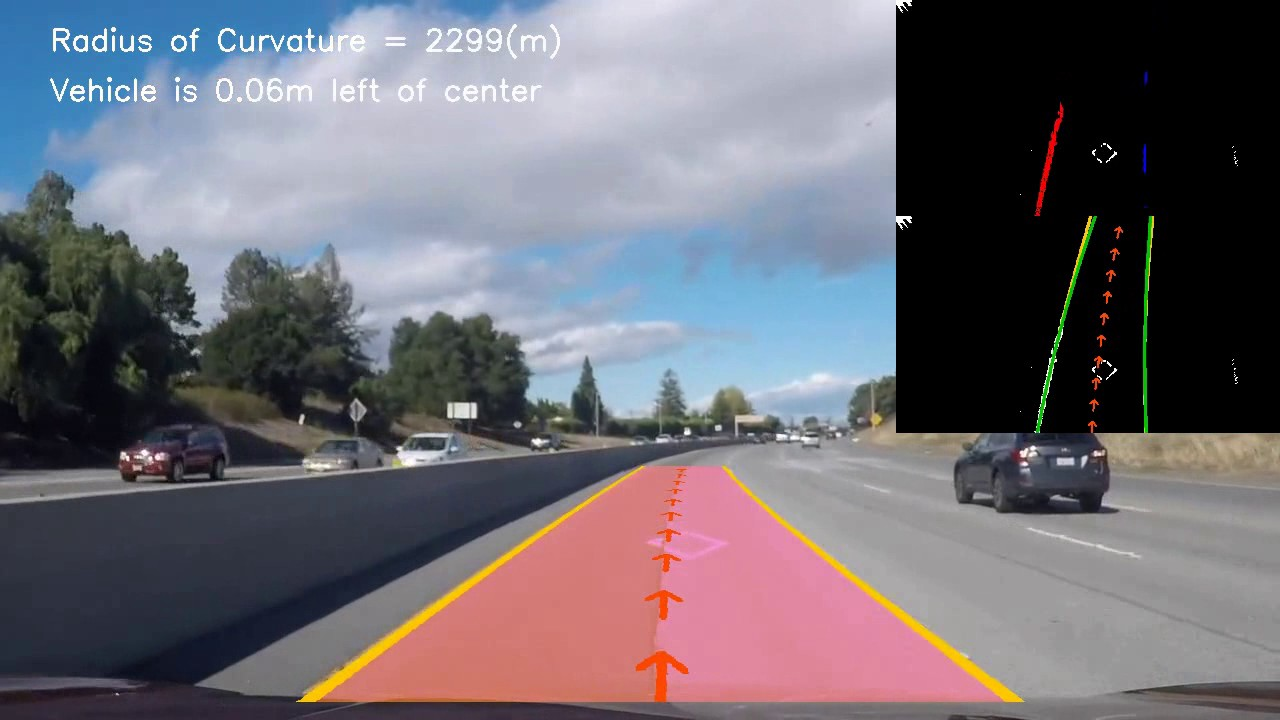
\includegraphics[width=\textwidth]{lanedetection.jpg}
    \caption{Lane Line Marking Detection using Deep Learning \cite{road}.}
    \label{fig:lanedetection}
\end{figure}


\subsubsection{On Road Object Detection}
In \cite{vision}, an energy minimization approach was presented for bounding box
proposal. These proposals were generated by exhaustively placing 3D bounding
boxes on the ground-plane, projecting them to the image plane and scoring them
via simple and efficiently computable image features including semantic and
object instance segmentation, context, shape features, and location priors to
score the boxes. Per-class weights were also learnt for these features using
S-SVM, adapting to each individual object class. On-road object detection mainly
concerns vehicle and pedestrian object classes. As listed in the KITTI database,
for car, pedestrian, and cyclist detections, all of the leading entries and
state of the art methods are based on deep learning schemes. Deep learning has
shown its superior performance as compared to conventional learning or feature
based approaches in the domain of obstacle detection. Let's review the deep
learning based approaches. Normally, the general pipeline for deep learning
approaches is that a set of proposal bounding boxes needs to be generated around
the input image, then each proposal box will be sent through the CNN network to
determine a classification (including background) and fine tune its bounding box
locations as well. The common methods for bounding box proposal are Selective
Search and EdgeBoxes, which both rely on inexpensive hand-crafted features and
economical inference schemes.

Faster-RCNN was the first deep learning scheme that unify both the
bounding box proposal and detection under the same network and achieved an
end-to-end training process. The network consists of two major parts: proposal
net and detection net, where these two nets share most of the CNN layers. The
output from the proposal net are the proposed bounding boxes, which is used as
the input to the detection net for recognition and bounding box fine tuning
processes.

\begin{figure}[h]
    \centering
    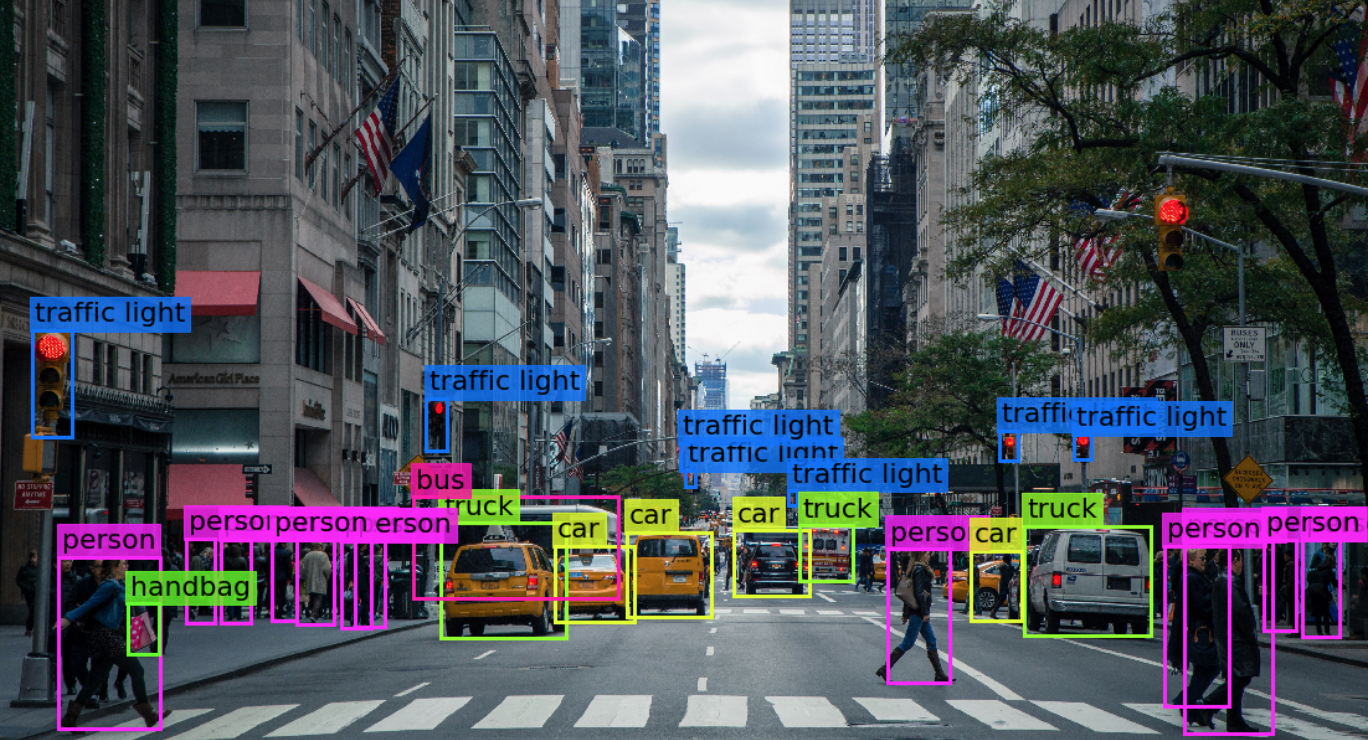
\includegraphics[width=0.7\textwidth]{onroadobjectdetection.png}
    \caption{On Road Object Detection using YOLO.}
    \label{fig:onroadobjectdetection}
\end{figure}

There also exists some other approaches in the literature to reduce the
processing time so that the deep learning approach can achieve (near) real time
performance, e.g., YOLO (You Only Look Once), SSD (Single Shot Detection). They
are able to process the images at more than 30 frames per second, varying with
the size of the network. However, the fast performance is achieved at the
expense of detection rate. As the technologies in both hardware and software
develop further, a better trade-off between the run time and detection rate can
be achieved.

\subsection{Fusion}

Different sensors have different strengths and weaknesses. Sensor fusion
techniques are required to make full use of the advantages of each sensor. In
the context of autonomous vehicle environment perception, LIDAR is able to
produce 3D measurements and is not affected by the illumination of the
environment, but it offers little information on objects’ appearances;
conversely, camera is able to provide rich appearance data with much more
details on the objects, but its performance is not consistent across different
illumination conditions; furthermore, camera does not implicitly provide 3D
information.

The techniques that have been applied to LIDAR and camera fusion can be roughly
divided into two main categories based on their fusion process locations,
including fusion at feature level (early stage, centralized fusion) and fusion
at decision level (late stage, decentralized fusion). Based on the fusion
mechanisms, they can be divided into the following categories: MRF/CRF based,
probability based, and deep learning based.

\subsection{Localization}

The localization module is responsible for estimating the self-driving car pose
(position and orientation) relative to a map or road (e.g., represented by curbs
or road marks). Most general-purpose localization subsystems are based on GPS.
However, by and large, they are not applicable to urban self- driving cars,
because the GPS signal cannot be guaranteed in occluded areas, such as under
trees, in urban canyons (roads surrounded by large buildings) or in tunnels.

Various localization methods that do not depend on GPS have been proposed in the
literature. They can be mainly categorized into three classes: LIDAR-based,
LIDAR plus camera-based, and camera-based. LIDAR-based localization methods rely
solely on LIDAR sensors, which offer measurement accuracy and easiness of
processing. However, despite LIDAR industry efforts to reduce production costs,
it still has a high price if compared to cameras. In typical LIDAR plus
camera-based localization methods, LIDAR data is used only to build the map, and
camera data is employed to estimate the self-driving car’s position relative to
the map, which reduces costs. Camera-based localization approaches are cheap and
convenient, even though typically less precise and/or reliable.

\begin{figure}[h]
    \centering
    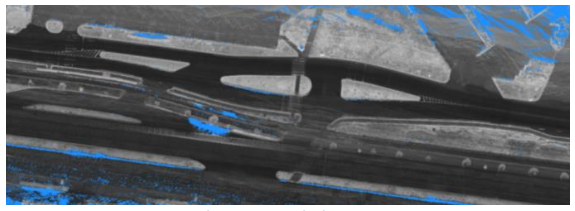
\includegraphics[width=0.9\textwidth]{remission.png}
    \caption{Remission Map}
    \label{fig:lidar}
\end{figure}
